\section{Feedforward neural networks}
Not really Bayesian, but whatever.
\subsection{Notation}
\begin{figure}[htb!]
    \centering
    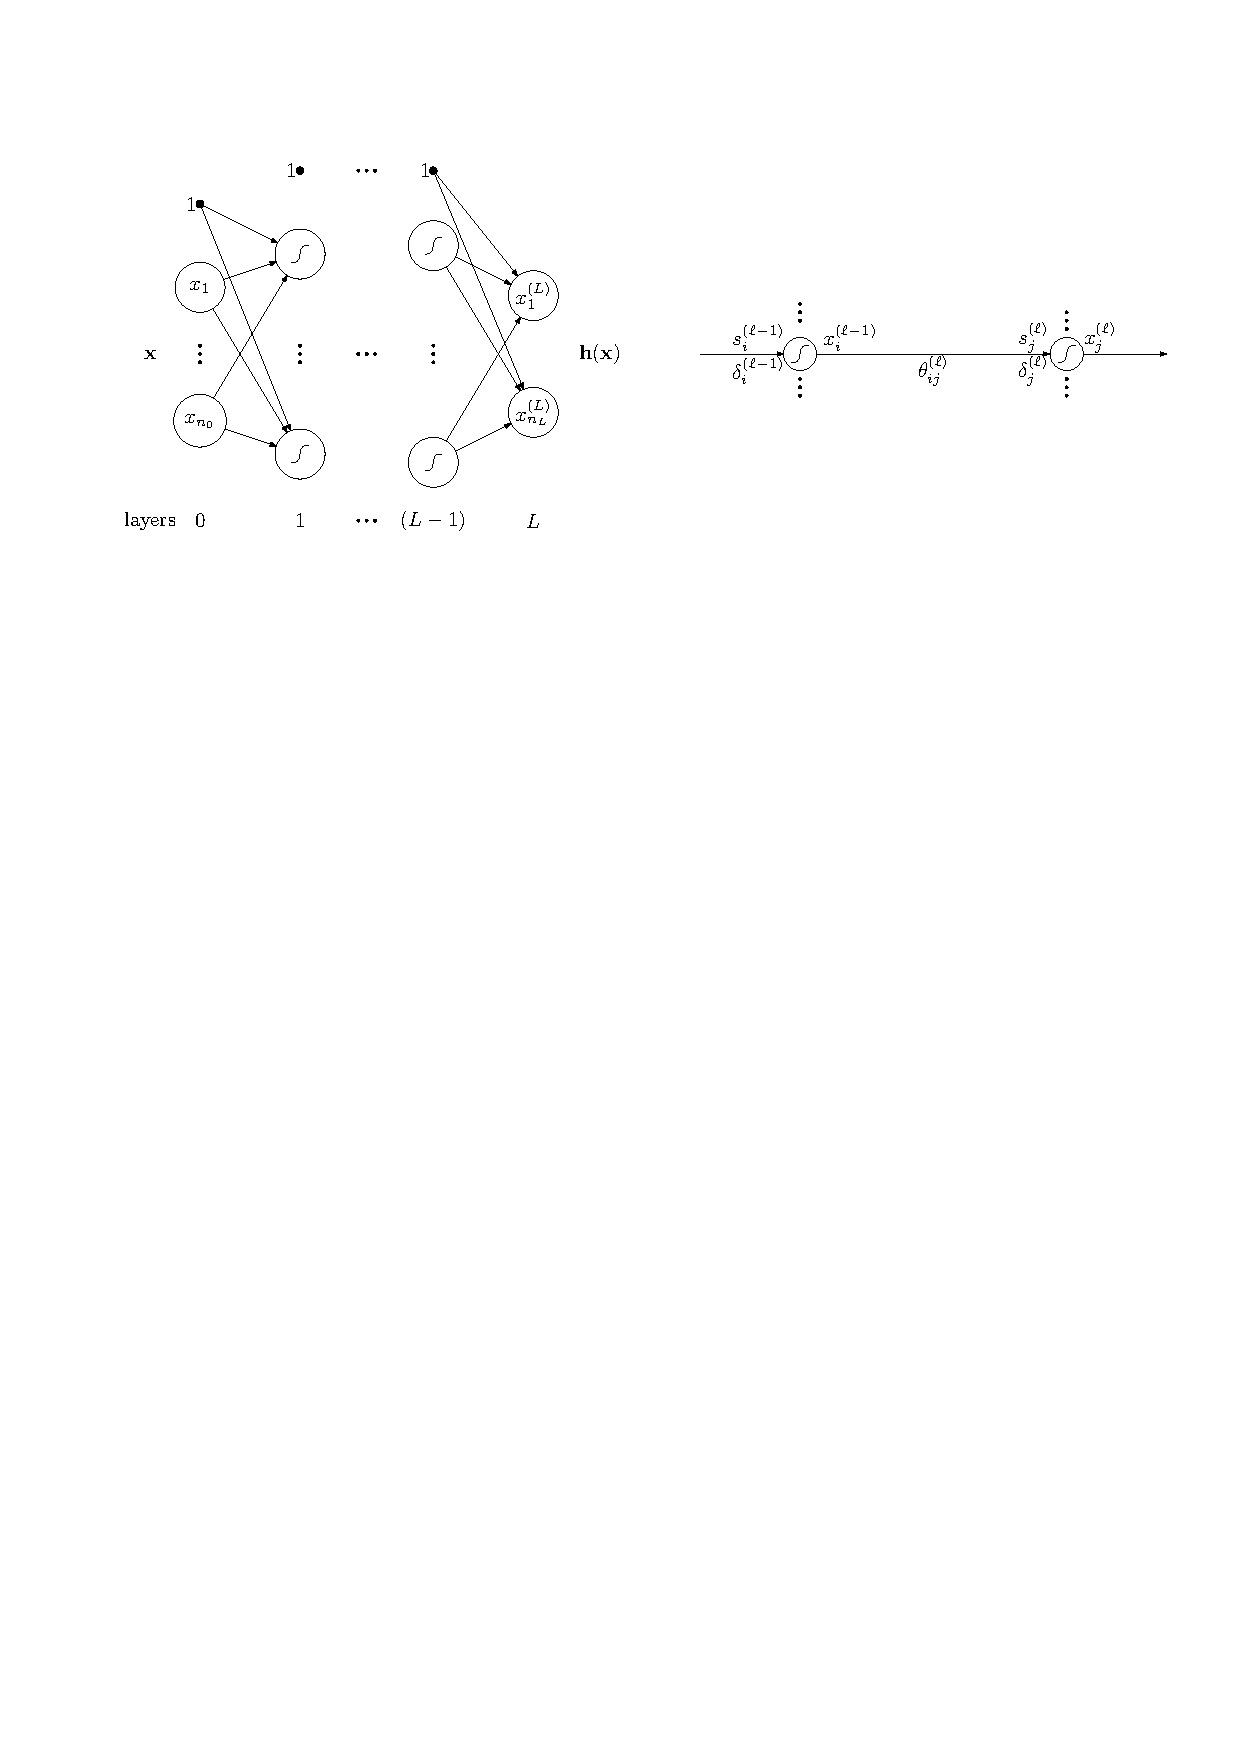
\includegraphics[width=1\textwidth]{nnets/figures/nnet}
    \caption{Feedforward neural network.}
\end{figure}

There are $L$ layers, $n_{\ell}$ at layer $\ell$. $\theta_{ij}^{(\ell)}$ is the weight where
\begin{itemize}
    \item layer $\ell = 1, \dotsc, L$
    \item input $i = 0, \dotsc, n_{\ell - 1}$ (includes the intercept)
    \item output $j = 1, \dotsc, n_\ell$.
\end{itemize}
The values of the neurons are
\begin{align}
    x_j^{(\ell)}    &= g\left(\sum_{i = 0}^{n_{\ell - 1}} \theta_{ij}^{(\ell)} x_i^{(\ell - 1)}\right) \label{eqn:nnets/feedforward/x-small}\\
                    &= g\left({\vec \theta_j^{(\ell)}}^T \vec x^{(\ell - 1)}\right) \\
                    &= g\left(s_j^{(\ell)}\right)
\end{align}
where
\begin{itemize}
    \item $x_0^{(\ell)} = 0, \ell = 1, \dotsc, L - 1$
    \item $g: \mathbb R \to \mathbb R$ is a differentiable, nonlinear \emph{activation function}
    \item $\vec \theta_j^{(\ell)} := (\theta_{0j}^{(\ell)}, \dotsc, \theta_{n_{\ell - 1}, j}^{(\ell)})^T \in \mathbb R^{n_{\ell - 1} + 1}$ are the weights from layer $(\ell - 1)$ to neuron $j$ in the layer $\ell$.
    \item $\vec x = (x_1, \dotsc, x_{n_0})^T$ is the input.
    \item $\vec x^{(\ell)} := (x_0^{(\ell)}, \dotsc, x_{n_\ell}^{(\ell)})^T \in \mathbb R^{n_\ell + 1}$ are the neurons in layer $\ell = 0, \dotsc L - 1$. Note that $\vec x^{(0)} = \left(x_0^{(0)}, \vec x^T\right)^T$.
    \item $\vec x^{(L)} := (x_1^{(L)}, \dotsc, x_{n_L}^{(L)})^T \in \mathbb R^{n_L}$ is the predicted output.
    \item $s_j^{(\ell)}$ is the \emph{signal} for the $j$-th neuron in the $\ell$-th layer. This gets fed into the \emph{activation function} to get the $(j, \ell)$-th neuron.
\end{itemize}
We can group the weights further, $\vec \Theta^{(\ell)} = (\vec \theta_1^{(\ell)}, \dotsc, \vec \theta_{n_\ell}^{(\ell)})^T \in \mathbb R^{n_\ell \times n_{\ell - 1}}$, so that
\begin{align}
    \vec x^{(\ell)} = g\left(\vec \Theta^{(\ell)} \vec x^{(\ell - 1)}\right) \label{eqn:nnets/feedforward/x}
\end{align}
Note the slight inaccuracy of notation in \eqref{eqn:nnets/feedforward/x}: we are overloading $g$ (for multivariable inputs and outputs) and also the left hand side should be $(x_1^{(\ell)}, \dotsc, x_{n_\ell}^{(\ell)})^T$ (it should not include the intercept term). We can finally group $\vec \Theta := (\vec \Theta^{(1)}, \dotsc, \vec \Theta^{(L)})$.

We define the mapping from input to output to be $\vec h$. The error on the example $(\vec x, \vec y)$ is $E(\vec \Theta)$ which is usually an analytic function of $\vec y$ and $\vec x^{(L)}$ (something like norm of the difference squared).

\subsection{Backpropagation algorithm}
We need to find $\grad_{\vec \Theta} E(\vec \Theta)$, which is finding $\frac{\partial E(\vec \Theta)}{\partial \theta_{ij}^{(\ell)}}$ for all $i, j, \ell$ (evaluated at the current values of neurons; we sometimes omit this for clarity). Since
\begin{align}
    \frac{\partial E(\vec \Theta)}{\partial \theta_{ij}^{(\ell)}} = \frac{\partial E(\vec \Theta)}{\partial s_j^{(\ell)}} \frac{\partial s_j^{(\ell)}}{\partial \theta_{ij}^{(\ell)}} \label{eqn:nnets/feedforward/backprop}
\end{align}
and
\begin{align}
                s_i^{(\ell)}                                                &= \sum_{i = 0}^{n_{\ell - 1}} \theta_{ij}^{(\ell)} x_i^{(\ell - 1)} \\
    \implies    \frac{\partial s_j^{(\ell)}}{\partial \theta_{ij}^{(\ell)}} &= x_i^{(\ell - 1)}
\end{align}
we only need
\begin{align}
    \delta_j^{(\ell)} := \frac{\partial E(\vec \Theta)}{\partial s_j^{(\ell)}}
\end{align}
to evaluate \eqref{eqn:nnets/feedforward/backprop}.

\paragraph{For the final layer.} We can find
\begin{align}
    \delta_j^{(L)}  &= \frac{\partial E(\vec \Theta)}{\partial s_j^{(L)}} \\
                    &= \frac{\partial E(\vec \Theta)}{\partial x_j^{(L)}} \frac{\partial x_j^{(L)}}{\partial s_j^{(L)}} \\
                    &= \frac{\partial E(\vec \Theta)}{\partial x_j^{(L)}} g'\left(s_j^{(L)}\right) \label{eqn:nnets/feedforward/delta-last}
\end{align}
analytically for $j = 1, \dotsc, n_L$.

\paragraph{For the layers before.} We can find
\begin{align}
    \delta_i^{(\ell - 1)}   &= \frac{\partial E(\vec \Theta)}{\partial s_i^{(\ell - 1)}}\at{x_i^{(\ell - 1)}} \\
                            &= \sum_{j = 1}^{n_\ell} \frac{\partial E(\vec \Theta)}{\partial s_j^{(\ell)}} \frac{\partial s_j^{(\ell)}}{\partial s_i^{(\ell - 1)}} \\
                            &= \sum_{j = 1}^{n_\ell} \frac{\partial E(\vec \Theta)}{\partial s_j^{(\ell)}} \frac{\partial s_j^{(\ell)}}{\partial x_i^{(\ell - 1)}} \frac{\partial x_i^{(\ell - 1)}}{\partial s_i^{(\ell - 1)}} \\
                            &= \sum_{j = 1}^{n_\ell} \delta_j^{(\ell)} \cdot \theta_{ij}^{(\ell)} \cdot g'\left(s_i^{(\ell - 1)}\right) \label{eqn:nnets/feedforward/delta-before}
\end{align}
recursively for $i = 1, \dotsc, n_{\ell - 1}$.

The algorithm becomes
\begin{algorithmbis}[Backpropagation algorithm (SGD)]\label{alg:nnets/feedforward/backprop}
    \begin{algorithmic}[1]
        \State Initialise $\vec \Theta$ at random.
        \Repeat
            \State Pick example $n \in \{1, \dotsc, N\}$ at random.
            \State Forward pass: compute all $x_j^{(\ell)}$'s using \eqref{eqn:nnets/feedforward/x-small}.
            \State Backward pass: compute all $\delta_j^{(\ell)}$'s using \eqref{eqn:nnets/feedforward/delta-last} and \eqref{eqn:nnets/feedforward/delta-before}.
            \State Update all $\theta_{ij}^{(\ell)}$'s:
                \begin{align}
                    \theta_{ij}^{(\ell)}    &\leftarrow \theta_{ij}^{(\ell)} - \eta\frac{\partial E(\vec \Theta)}{\partial \theta_{ij}^{(\ell)}} \\
                                            &= \theta_{ij}^{(\ell)} - \eta x_i^{(\ell - 1)} \delta_j^{(\ell)}
                \end{align}
        \Until{it is time to stop.}
        \State Return the final weights $\vec \Theta$.
    \end{algorithmic}
\end{algorithmbis}

\subsection{Full specifications}
In order to fully specify the network and the backpropagation algorithm, we need to specify \emph{activation functions} $g$, their derivatives $g'$, the error $E$ and its derivatives $\frac{\partial E(\vec \Theta)}{\partial x_j^{(L)}}$. Then we can arbitrarily mix and match activation functions and error functions to give us the required output, etc.

\subsubsection{Sigmoid activation}
For $[0, 1]$ output:
\begin{align}
    g(x) &= \frac{1}{1 + \exp(-x)} \\
    g'(x) &= g(x)(1 - g(x)).
\end{align}

\subsubsection{Identity activation}
For $\mathbb R$ output:
\begin{align}
    g(x) &= x \\
    g'(x) &= 1.
\end{align}

\subsubsection{Softmax activation}
For vector output that sums to one:
\begin{align}
    g(\vec x)_i                                 &= \frac{\exp(x_i)}{\sum_j \exp(x_j)} \\
    \frac{\partial g(\vec x)_i}{\partial x_j}   &= g(\vec x)_i (\delta_{ij} - g(\vec x)_j).
\end{align}
Note that $\delta_{ij}$ is the Kronecker delta function and $= 1$ if $i = j$ and $= 0$ otherwise.

\subsubsection{Exponential activation}
For $\mathbb R^+$ output:
\begin{align}
    g(x) &= \exp(x) \\
    g'(x) &= \exp(x).
\end{align}

\subsubsection{Tanh activation}
For $[0, 1]$ output:
\begin{align}
    g(x)    &= \tanh(x) \\
            &= \frac{\exp(x) - \exp(-x)}{\exp(x) + \exp(-x)} \\
    g'(x)   &= 1 - \tanh^2(x).
\end{align}

\subsubsection{Rectifier activation}
For $R^+$ output:
\begin{align}
    g(x)    &= \max(0, x) \\
    g'(x)   &=
        \begin{cases}
            0 & \text{if } x < 0 \\
            1 & \text{if } x > 0
        \end{cases}.
\end{align}
Use whatever for $g'(0)$.

\subsubsection{Squared norm error}
\begin{align}
    E(\vec \Theta)  &= \frac{1}{2}\left\|\vec x^{(L)} - \vec y \right\|^2 \\
                    &= \frac{1}{2}\left(\vec x^{(L)} - \vec y\right)^T \left(\vec x^{(L)} - \vec y\right) \\
    \grad_{\vec x^{(L)}} E(\vec \Theta) &= \left(\vec x^{(L)} - \vec y\right)
\end{align}

\subsection{Feedforward neural networks for conditional density estimation}
\begin{figure}[htb!]
    \centering
    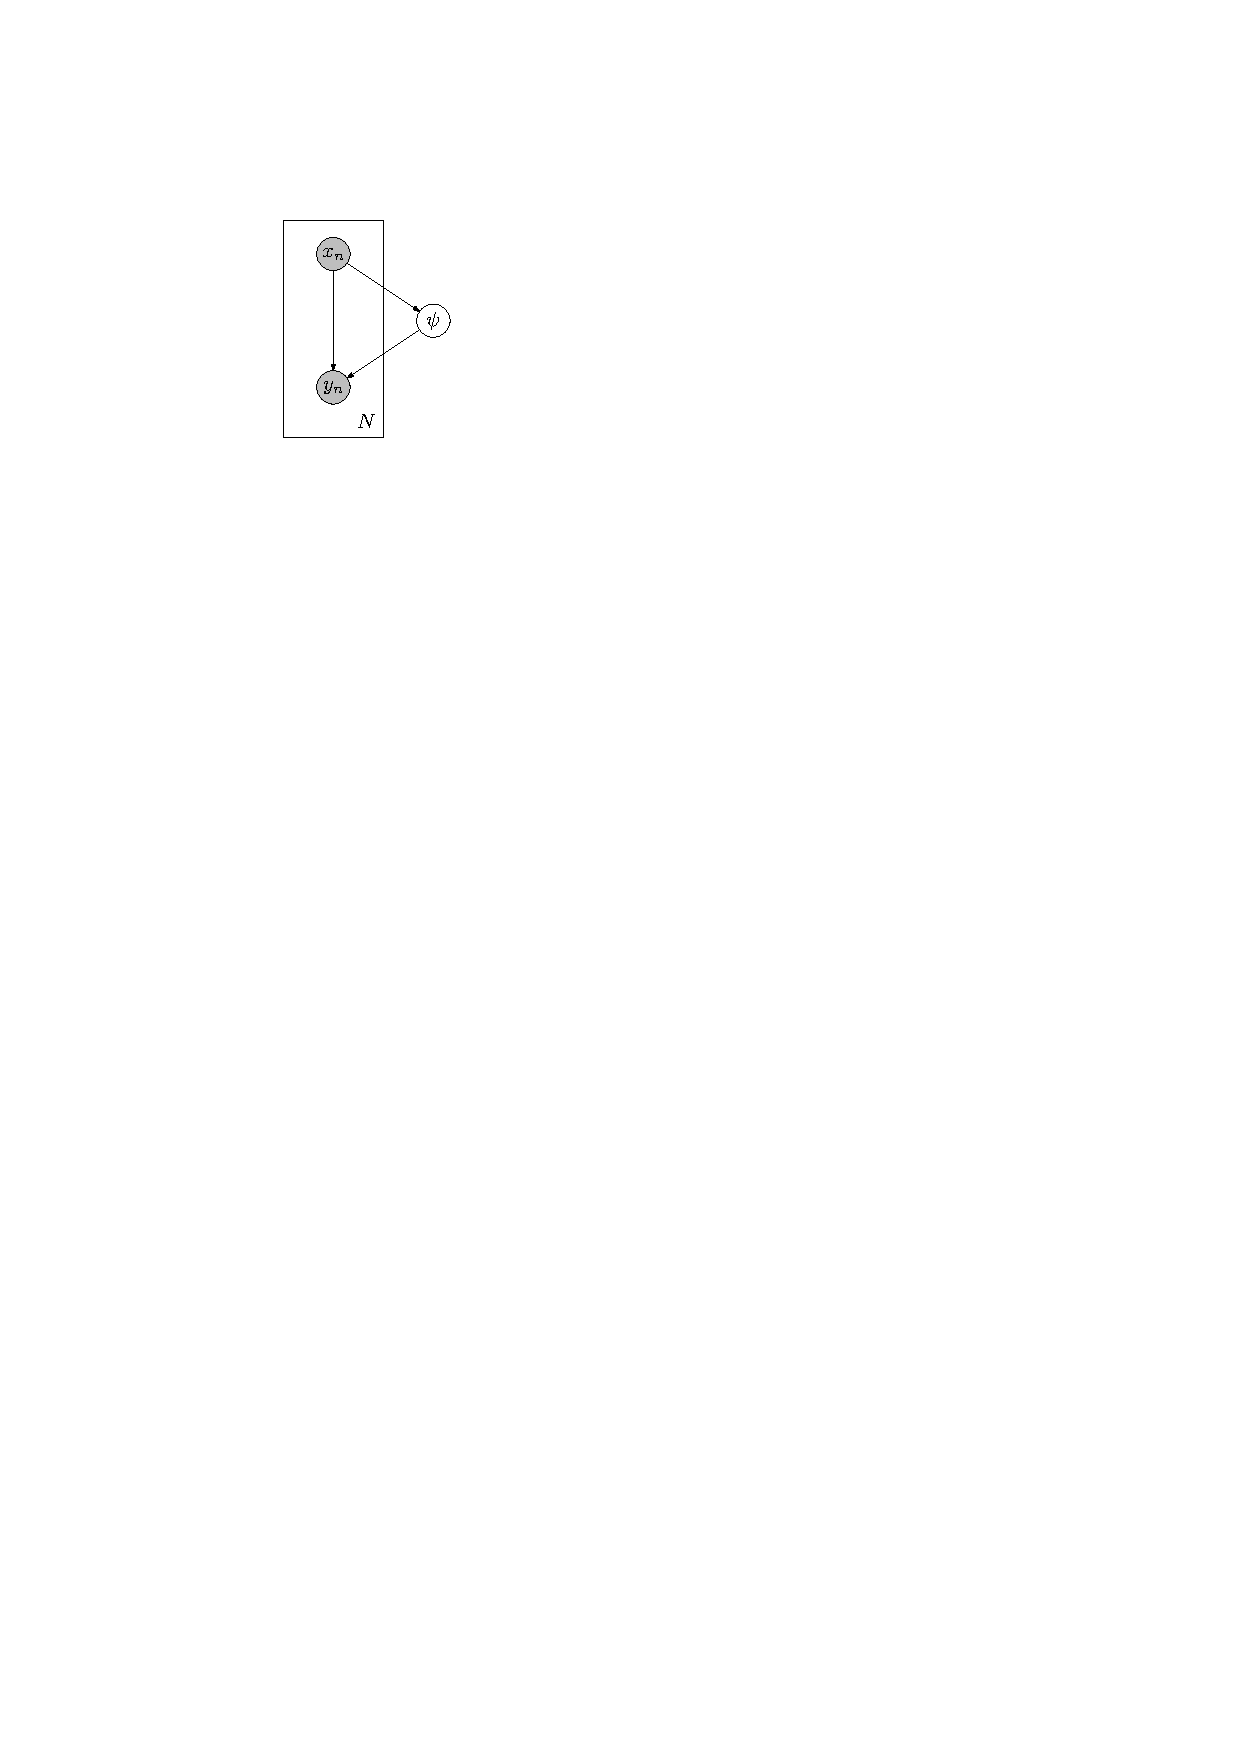
\includegraphics{nnets/figures/conditional-density-estimation}
    \caption{Graphical model for conditional density estimation.}
    \label{fig:nnets/feedforward/cond}
\end{figure}
We are interested in estimating $y \given x$ using a neural network using training data $\{x_n, y_n\}$. What can set up the following generative model
\begin{align}
    \psi &:= \eta(x_n) \\
    y_n \given x_n, \psi &\sim F(x_n, \psi)
\end{align}
where $\eta$ is our neural network and $F$ is some generative model with some density function $f$. By maximising the likelihood
\begin{align}
    \mathcal L(\psi) = \prod_n f(y_n \given x_n, \psi)
\end{align}
we can find the MLE estimate of $\psi$. This is equivalent to setting the error function of the neural network $\eta$ to be the negative log-likelihood of one data point:
\begin{align}
    E_n(\vec \Theta)    &= -\log f(y_n \given x_n, \psi)
\end{align}
where $\vec \Theta$ are the weights of the neural network. If we can design a generative model $F$ in such a way that we can calculate the derivatives $\frac{\partial E_n(\vec \Theta)}{\partial x_j^{(L)}}$, then we are done (SGD will minimise $\sum_n E_n$ which is total negative log-likelihood). We need to mix and match the activation functions for the last layer to match the support of $\psi$.

\subsubsection{Example}
Let the generative model be
\begin{align}
    f(y \given x, \psi) &= \Gauss(y \given x, \psi) \\
                        &= \Gauss(y \given m, \sigma^2)
\end{align}
where
\begin{align}
    \psi = (m, \sigma).
\end{align}

Let the input to the a 2 layer (1 input layer, 1 hidden layer, 1 output layer) neural network be $\vec x = (x_1, x_2) \in \mathbb R^2$ and the output be
\begin{itemize}
    \item $x_1^{(2)} \in \mathbb R$ which is approximating $m$, and
    \item $x_2^{(2)} \in \mathbb R^+$ which is approximating $\sigma$.
\end{itemize}

Our negative log-likelihood for one data point a.k.a. error function is
\begin{align}
    E(\vec \Theta)  &= -\log\Gauss\left(y \given x_1^{(2)}, \left(x_2^{(2)}\right)^2\right) \\
                    &= -\log \frac{1}{x_2^{(2)} \sqrt{2\pi}} \exp{-\frac{(x_1^{(2)} - y)^2}{2\left(x_2^{(2)}\right)^2}} \\
                    &= \log(\sqrt{2\pi}) + \log(x_2^{(2)}) + \frac{(x_1^{(2)} - y)^2}{2\left(x_2^{(2)}\right)^2}
\end{align}
and the derivatives are
\begin{align}
    \frac{\partial E}{\partial x_1^{(2)}}  &= 2\left(x_1^{(2)} - y\right) \\
    \frac{\partial E}{\partial x_2^{(2)}}  &= \frac{1}{x_2^{(2)}} - \left(x_1^{(2)} - y\right)^2\left(x_2^{(2)}\right)^{-3} \\
                                    &= \frac{1}{x_2^{(2)}}\left(1 - \frac{(x_1^{(2)} - y)^2}{\left(x_2^{(2)}\right)^2}\right).
\end{align}
We choose the identity and exponential activation functions for $m$ and $\sigma$ respectively.